\section{User app}

**** desccribir un poco el funcionamiento de react native y su implementacion con componentes nativos. Describir las librerias utilizadas para la aplicacion movil

\begin{itemize}
	\item fetch
	\item react-native-jwt
\end{itemize}

*** mencionar los archivos que son importantes para el proyecto


\begin{figure}[htbp]
	\centerline{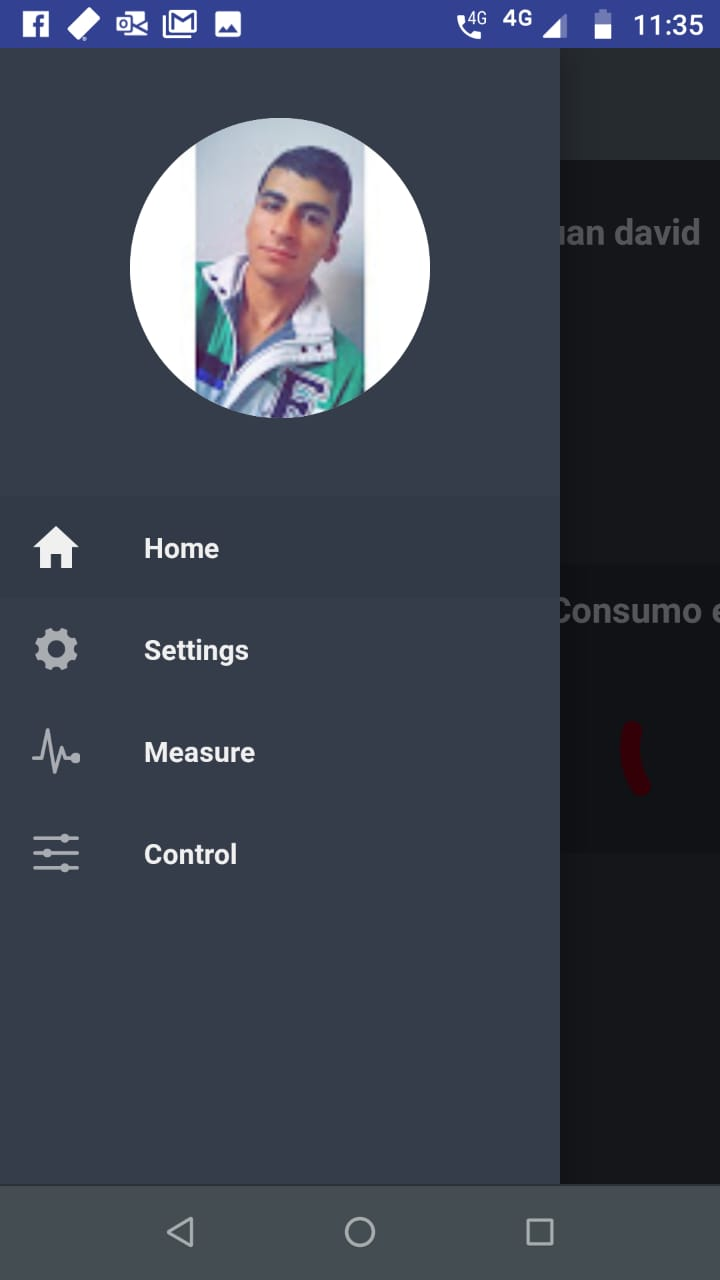
\includegraphics[width=8.5cm]{./figuras/mobile_menu.jpeg}}
	\caption{El menu desplegable con las aplicaciones actualmente desplegadas}
	\label{fig_17}
\end{figure}

*** hablar e la escalabilidad teniendo en cuenta la organizacion de la app


\subsection{Requerimientos Funcionales}

*** introducir los requerimientos funcionales de la plataforma y su importancia


\begin{enumerate}
	\item \textsl{"El usuario debe poder acceder a la informacion medida en tiempo real"} description
	
	\begin{figure}[htbp]
		\centerline{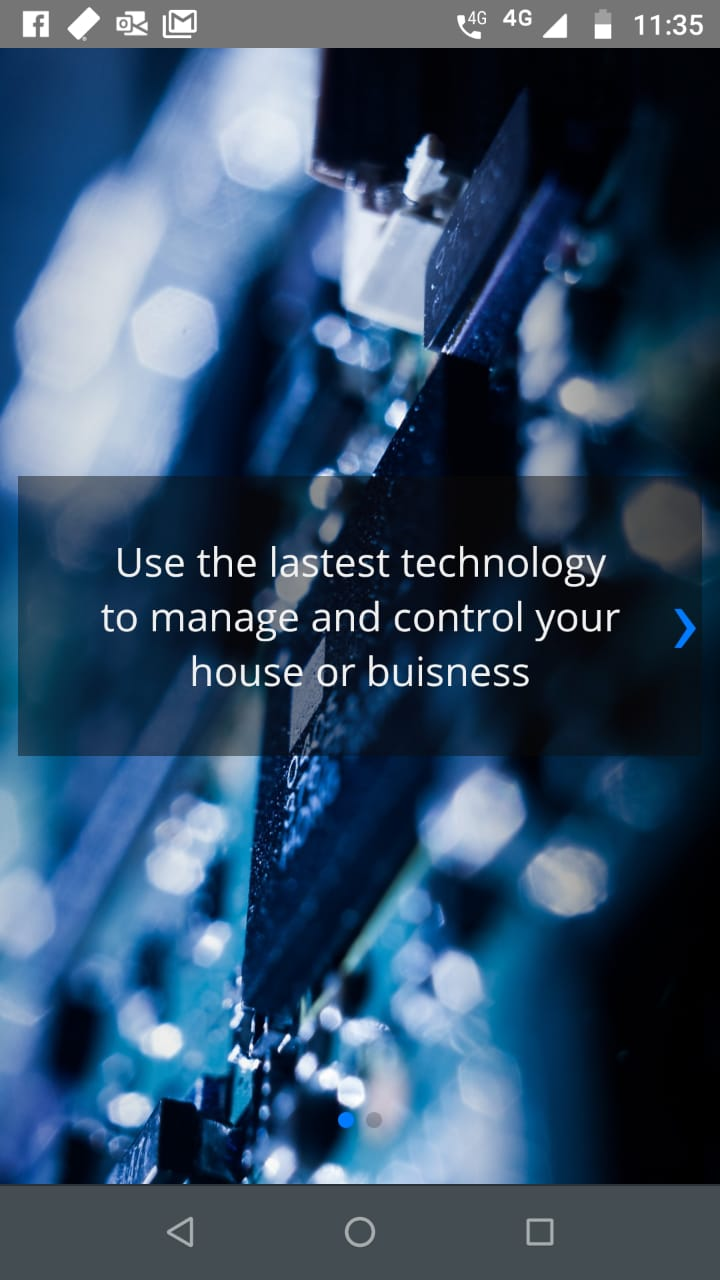
\includegraphics[width=8.5cm]{./figuras/mobile_intro1.jpeg}}
		\caption{Escena de bienvenida 1}
		\label{fig_12}
	\end{figure}
	
	\item \textsl{"el usuario debe poder acceder al historico del mes y la relacion de sus gastos con ellos"} description
	
	
	\begin{figure}[htbp]
		\centerline{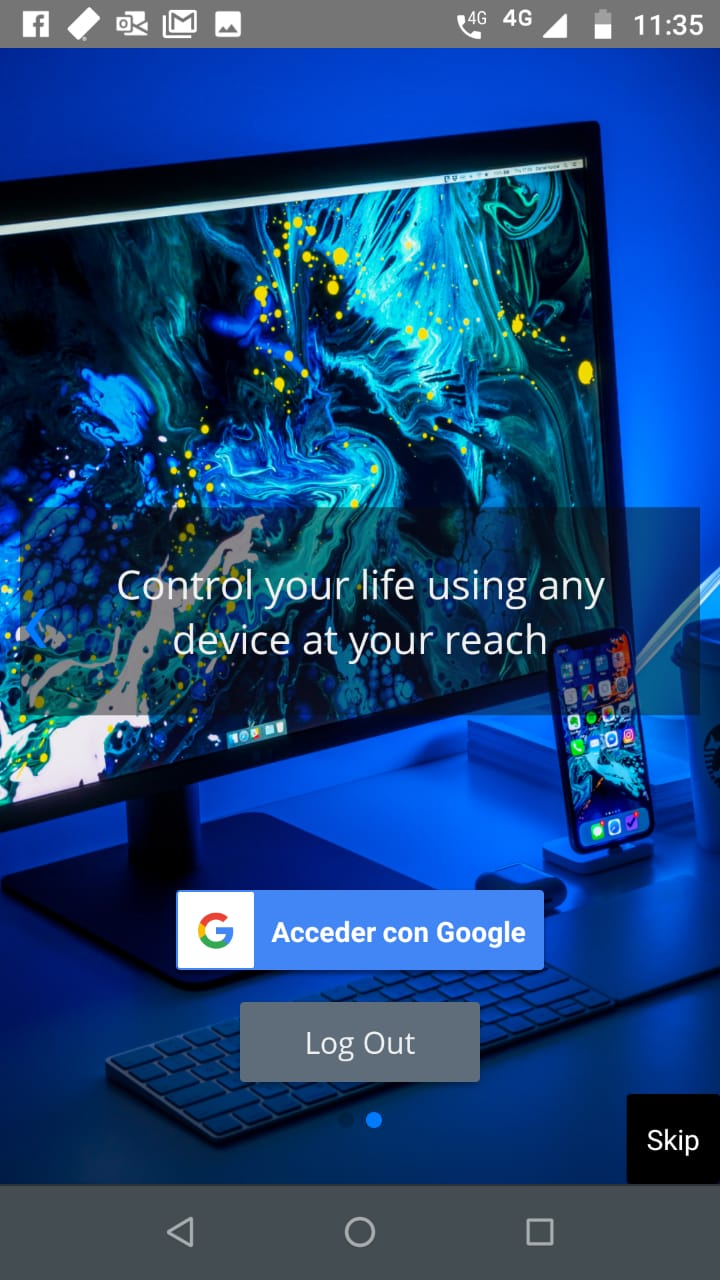
\includegraphics[width=8.5cm]{./figuras/mobile_intro2.jpeg}}
		\caption{Escena de logg in}
		\label{fig_13}
	\end{figure}
	
	\item  \textsl{"el usuario debe ser capaz de cambiar los parametros de configuraciones establecidos por defecto para la vivienda del solar decathlon"} description 
	
	
	\begin{figure}[htbp]
		\centerline{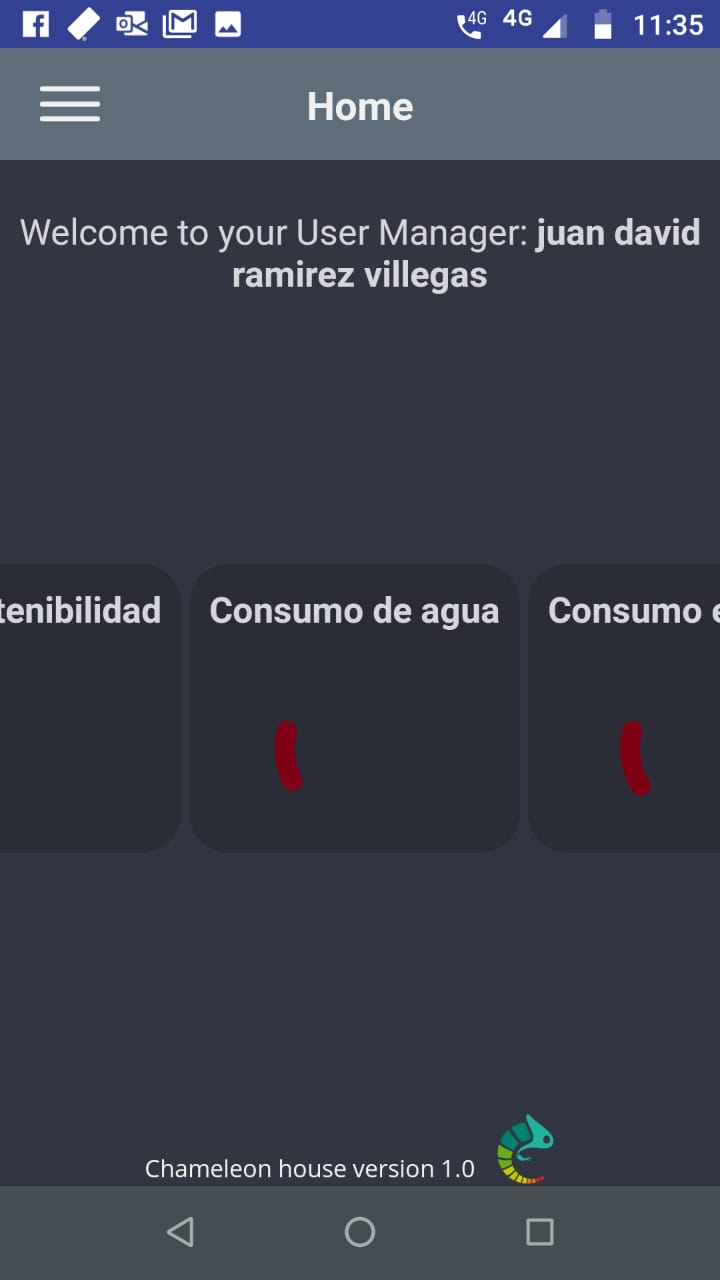
\includegraphics[width=8.5cm]{./figuras/mobile_home.jpeg}}
		\caption{Escena para a visualizacion del consumo historico}
		\label{fig_14}
	\end{figure}
	
	
	\item  \textsl{"la aplicacion notificara al usuario cuando la factura este vencida"} description
	 \begin{figure}[htbp]
	 	\centerline{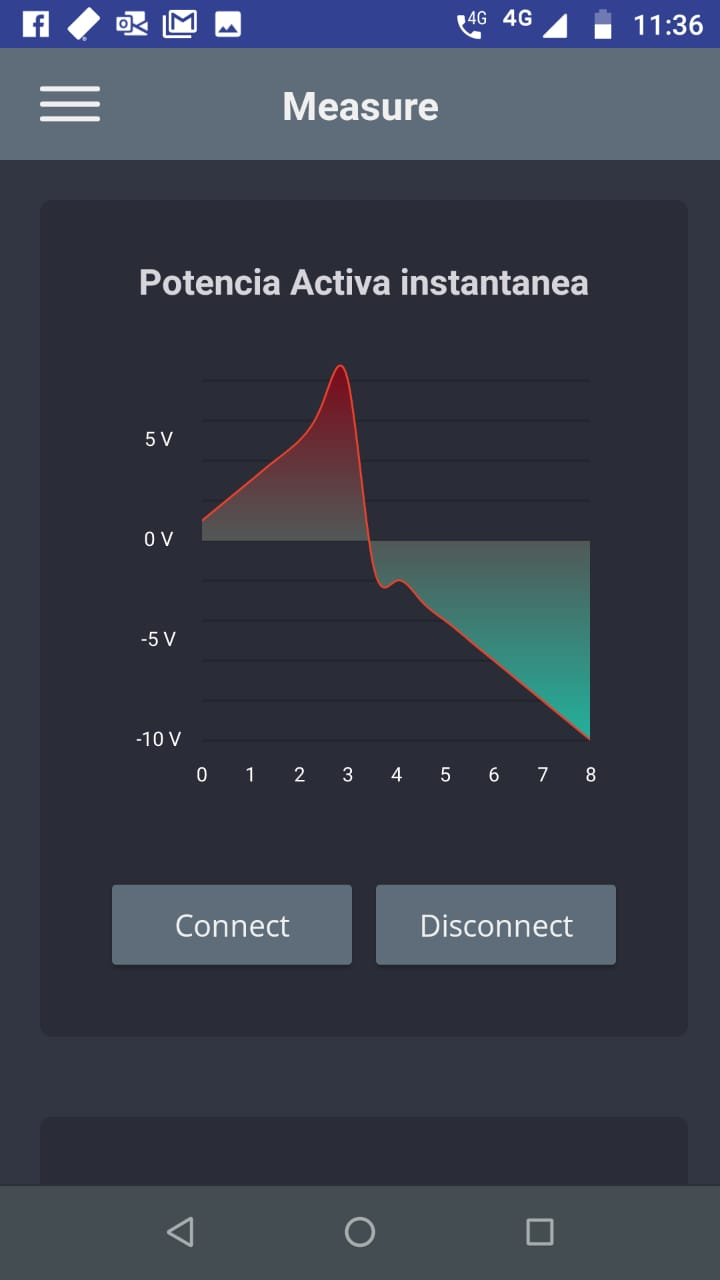
\includegraphics[width=8.5cm]{./figuras/mobile_measure.jpeg}}
	 	\caption{Escena para la medicion en tiempo real de las variables}
	 	\label{fig_15}
	 \end{figure}
	 
	 
	
	 
	\item \textsl{"el usuario debe ser capaz de poder ver su impacto ambiental basado en datos cualitativos y cuantitativos "} description
	
	\begin{figure}[htbp]
		\centerline{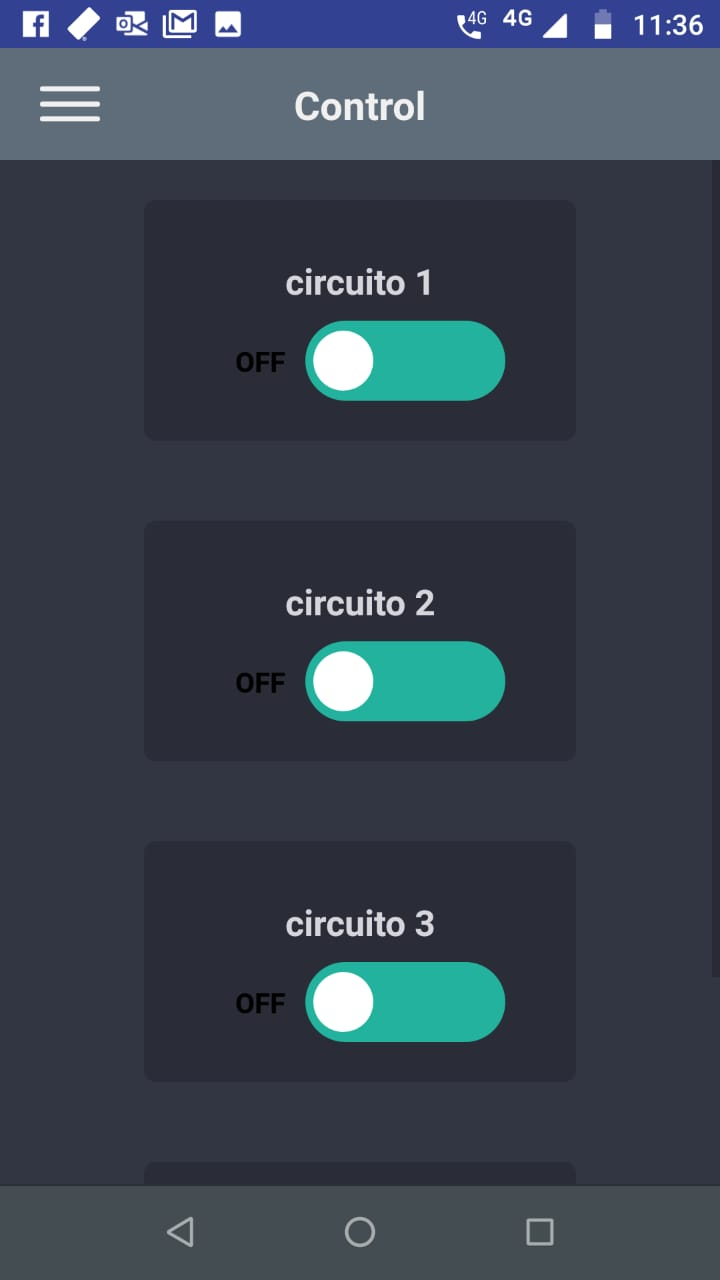
\includegraphics[width=8.5cm]{./figuras/mobile_control.jpeg}}
		\caption{Escena para el control de los circuitos de la vivienda}
		\label{fig_16}
	\end{figure}

	\item \textsl{"El sistema debe ser capaz de notificar las perdidas electricas y por consiguiente economicas de un mal uso de los horarios establecidos por defecto:"}
\end{enumerate}



\begin{figure}[htbp]
	\centerline{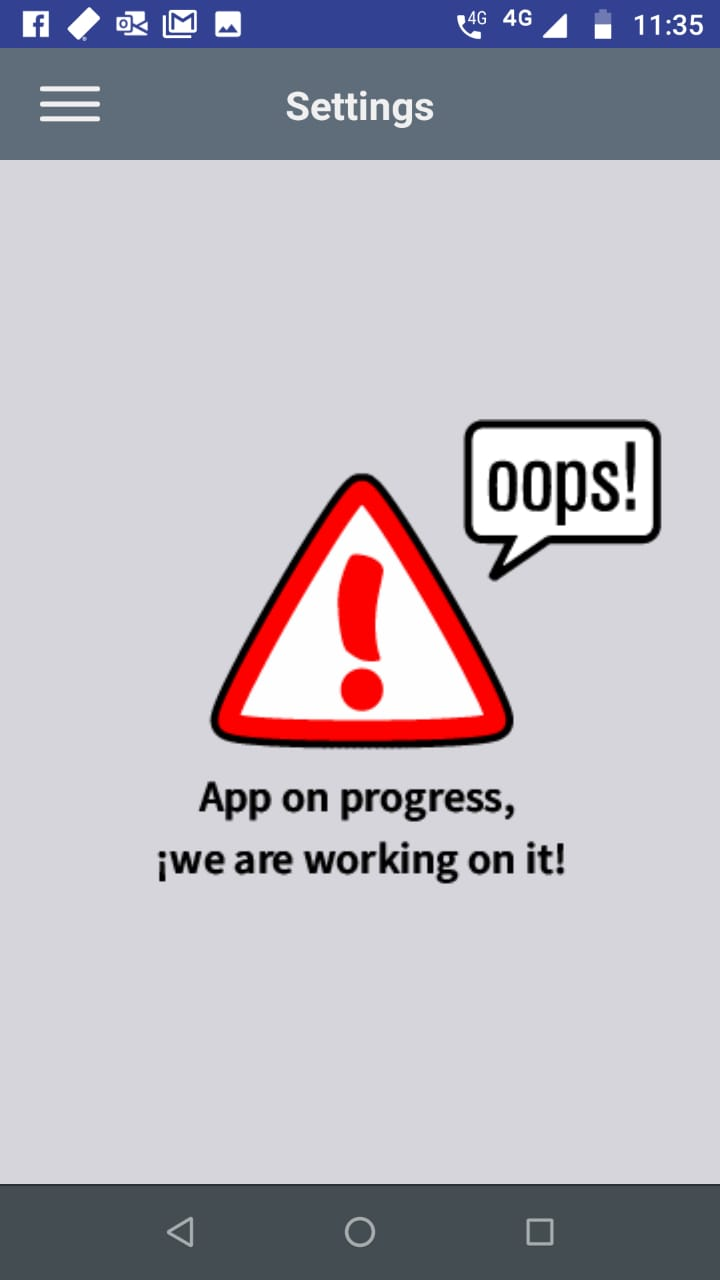
\includegraphics[width=8.5cm]{./figuras/mobile_settings.jpeg}}
	\caption{Escena de configuraciones, actualmente no disponible}
	\label{fig_18}
\end{figure}



\subsection{Funciones adicionales}

*****Funciones adicionales


\begin{enumerate}
	\item \textbf{Handler remoto:} description
	
	\item \textbf{Sistema de almacenamiento local:} description
	
	\item \textbf{Ajustes de configuracion} description
	
\end{enumerate}

\subsection{Algoritmos Utilizados}

**** describir la naturaleza de un entorno de programacion orientado a relaciones como los algoritmos eran codificados en funcion de cambiar una propiedad del elemento

\subsubsection{Scheduler Handler}

***incluir diagrama del algoritmo y explicarlo 

\subsubsection{Remote Mode Handler}

***incluir diagrama del algoritmo y explicarlo 